\normaltrue
\correctionfalse

%\UPSTIidClasse{11} % 11 sup, 12 spé
%\newcommand{\UPSTIidClasse}{12}

\exer{Mouvement RT  $\star$ \label{C2:08:05}}
\setcounter{numques}{0}
\UPSTIcompetence[2]{C2-08}
\UPSTIcompetence[2]{C2-09}
\index{Compétence C2-08}
\index{Compétence C2-09}
\index{Torseur cinétique}
\index{Torseur dynamique}
\index{Mécanisme à 1 rotation et 1 translation}
\ifcorrection
\else
\textbf{Pas de corrigé pour cet exercice.}
\fi

\ifprof
\else
Soit le mécanisme suivant. On a $\vect{AB}=\lambda(t)\vect{i_1}$. De plus :
\begin{itemize}
\item $G_1$ désigne le centre d'inertie de \textbf{1} et $\vect{AG_1}=L_1\vect{i_1}$, on note $m_1$ la masse de \textbf{1} et $\inertie{G_1}{1}=\matinertie{A_1}{B_1}{C_1}{0}{0}{0}{\bas{1}}$; 
\item $G_2=B$ désigne le centre d'inertie de \textbf{2}, on note $m_2$ la masse de \textbf{2} et $\inertie{G_2}{2}=\matinertie{A_2}{B_2}{C_2}{0}{0}{0}{\bas{2}}$.
\end{itemize}
\begin{center}
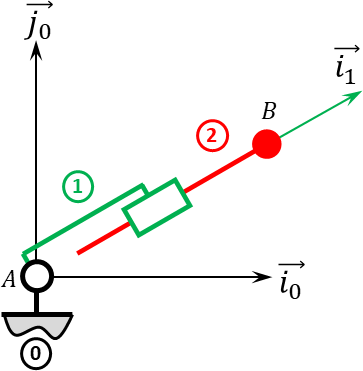
\includegraphics[width=\linewidth]{05_RT_01}
\end{center}
\fi

\question{Exprimer le torseur dynamique $\torseurdyn{1}{0}$ en $B$.}
\ifprof
\else
\fi

\question{Déterminer $\vectmd{A}{1+2}{0}\cdot \vect{k_0}$}
\ifprof
\else
\fi

\ifprof
\else
\begin{flushright}
\footnotesize{Corrigé  voir \ref{C2:08:05}.}
\end{flushright}%
\fi